\chapter{PROCESAMIENTO DEL LENGUAJE NATURAL Y CONJUNTO DE DATOS}\label{chp-controlIoT}
El Procesamiento del Lenguaje Natural (PLN) constituye un campo multidisciplinario que se centra en la interacción entre las computadoras y el lenguaje humano. Su objetivo principal es ayudar a las máquinas a comprender, interpretar y generar lenguaje natural de manera similar a la capacidad humana. En este capítulo, se proporciona una visión detallada que abarca desde los fundamentos teóricos hasta las técnicas modernas y las aplicaciones prácticas del PLN, lo que permite comprender tanto el estado actual como el potencial de este campo. Además, dada la escasez de conjuntos de datos que contienen lenguaje ofensivo en español, particularmente aquellos enfocados en el español de Bolivia, se detalla la creación de un conjunto de datos específico. Este conjunto de datos resultara sumamente útil para ser empleado por los modelos de aprendizaje automático propuestos en este contexto.

\section{DEFINICIÓN}
El Procesamiento del Lenguaje Natural (PLN) emerge de la combinación entre la inteligencia artificial y la lingüística. A diferencia de las diversas tareas que pueden tratar el aprendizaje automático o el aprendizaje profundo, el pnl se enfoca en tareas relacionadas con cualquier lenguaje o idioma, que los seres humanos utilicen para comunicarse de manera cotidiana, ya sea oral o escrita, este tipo de lenguaje es inherente a las culturas y evoluciona orgánicamente a lo largo del tiempo.

Vajjala define el PLN como ``un área de la informática que se enfoca en métodos para analizar, modelar y comprender el lenguaje humano. Prácticamente toda aplicación inteligente que implica el lenguaje humano tiene raíces en el PLN'' \cite[p. 4]{vajjala2020practical}.
 
El procesamiento del lenguaje natural, el aprendizaje profundo y el aprendizaje automático son subcampos de la Inteligencia Artificial que, de hecho, se superponen  entre ellos, ver Figura \ref{fig:nlp1}.Ya que estas disciplinas colaboran entre sí e incluso sirven como base la una a la otra, como ocurre con el aprendizaje automático y el aprendizaje profundo, e igualmente  muchos modelos de lenguaje hacen uso tanto del aprendizaje profundo como de técnicas tradicionales del aprendizaje automático. Sin embargo esto no evita que cada una de estas disciplinas tenga su área específica de estudio. Como el PLN que, se concentra en el análisis y comprensión del lenguaje humano, explorando diversas técnicas para estos propósitos.

\begin{figure}
	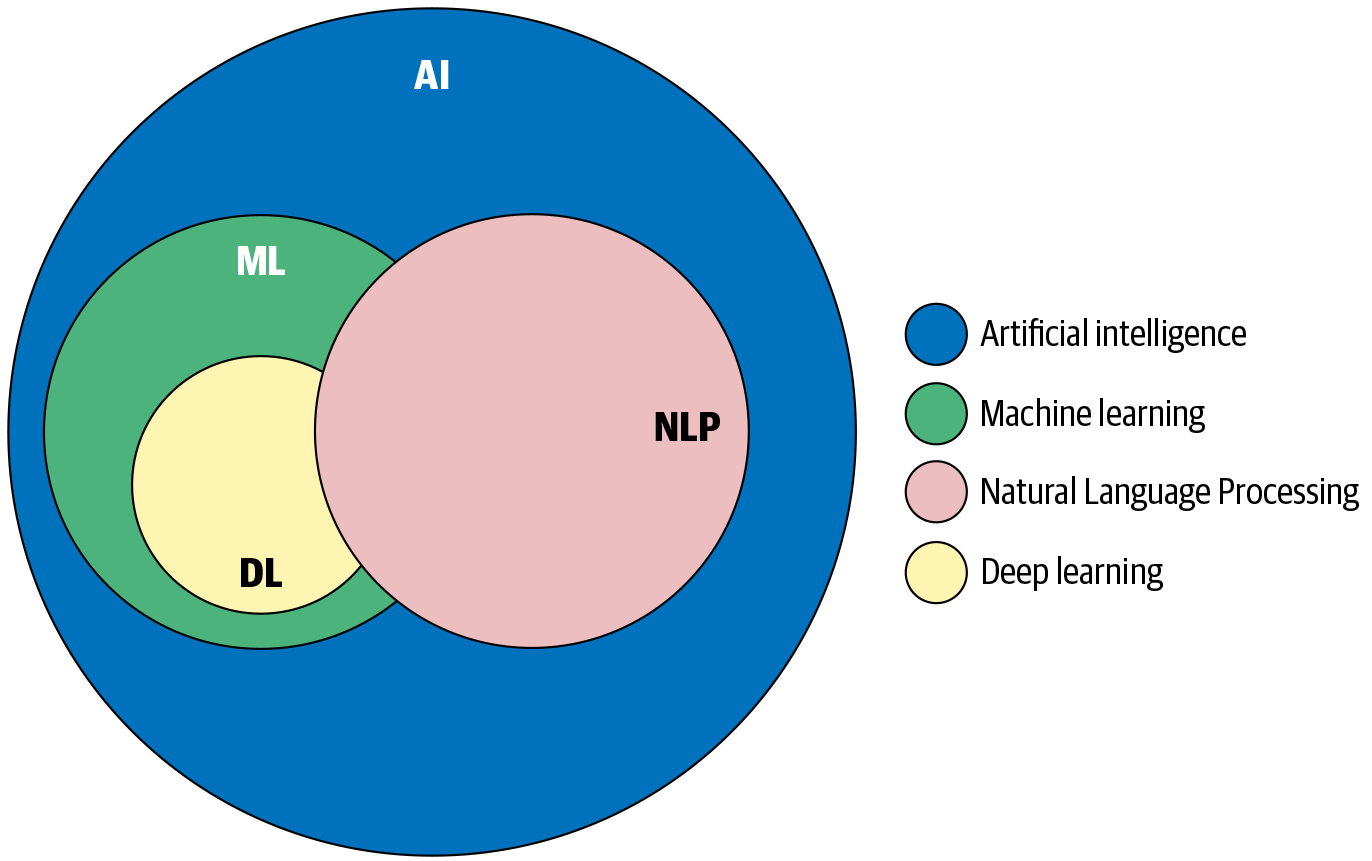
\includegraphics[width=0.65\textwidth]{capitulo3/figuras/nlp1.png}
	\caption{Como NLP, ML, y DL se relacionan}
	\floatfoot{Fuente: Practical natural language processing: A comprehensive guide to building real-world NLP systems \cite[p. 15]{vajjala2020practical} } 
	\label{fig:nlp1}
\end{figure}

\section{BREVE HISTORIA DEL PLN}
El Procesamiento del Lenguaje Natural (PLN) ha evolucionado desde los años 50, cuando Alan Turing planteó la posibilidad de evaluar la inteligencia de una máquina a través de conversaciones humanas en un artículo publicado en 1950 llamado ``Computing Machinery and Intelligence'' (Máquinas de computación e inteligencia) \cite{turing2009computing}. En la década de los 60, se desarrollaron los primeros programas de traducción automática y análisis gramatical. Uno de los primeros sistemas de PLN fue el ``ELIZA'', creado por Joseph Weizenbaum en 1966, que simulaba una conversación terapéutica \cite{weizenbaum1966eliza}.

En los años 70, la influencia de la Gramática Generativa Transformacional de Noam Chomsky fue significativa en el ámbito del Procesamiento del Lenguaje Natural (PLN). Esta teoría lingüística propuesta por Chomsky en las décadas anteriores buscaba establecer reglas abstractas y universales para explicar cómo se generan y estructuran las oraciones en cualquier lengua \cite{chomsky1970remarks}.

En ese período, los modelos de PLN estaban fuertemente influenciados por esta perspectiva basada en reglas. Se intentaba aplicar las ideas de la gramática generativa a la comprensión del lenguaje natural mediante la creación de sistemas computacionales que imitaran, en cierta medida, las reglas y principios gramaticales identificados por Chomsky. Estos sistemas se centraban en la construcción de reglas para analizar y procesar el lenguaje.

En los 80 hubo un cambio en el enfoque utilizado en los sistemas de PLN. Se adoptaron sistemas basados en el conocimiento y la codificación manual de reglas. En lugar de depender únicamente de los principios gramaticales generales, se codificaba manualmente reglas y patrones lingüísticos que se consideraban relevantes para las tareas específicas

El avance hacia los 90 trajo consigo la introducción de métodos estadísticos y basados en el aprendizaje automático en el PLN, junto con el crecimiento de la web que impulsó la necesidad de herramientas de búsqueda y análisis de texto a gran escala.

Desde el año 2000 en adelante, el PLN se ha expandido enormemente y se ha convertido en un campo multidisciplinario que incorpora el aprendizaje profundo, modelos basados en la estadística, el procesamiento de grandes volúmenes de datos (big data) y la aplicación de técnicas avanzadas en áreas como la comprensión del lenguaje, la traducción automática y los chatbots.

Esta rápida evolución continúa en la actualidad, con el PLN jugando un papel crucial en numerosas aplicaciones, desde motores de búsqueda hasta asistentes virtuales y análisis de sentimientos en redes sociales.

\section{TAREAS DE PLN}
El Procesamiento del Lenguaje Natural  abarca una gran variedad de tareas que se han vuelto imprescindibles para las personas, las mismas que  nos muestran una increíble evolución en la aplicabilidad de esta disciplina . Algunas de las tareas más comunes en PLN son:

\begin{itemize}

	\item Clasificación de Texto: Esta es una de las tareas más populares, se encarga de asignar etiquetas o categorías a un texto dado. Ejemplos incluyen la detección de spam en correos electrónicos o la clasificación de noticias por tema.

	\item Extracción de Información: Implica identificar y extraer información específica de textos, como nombres de personas, ubicaciones, fechas, etc., desde artículos o documentos.

	\item Análisis de Sentimientos: Determina la actitud emocional detrás de un texto, ya sea positiva, negativa o neutral. Es útil para evaluar opiniones en redes sociales, reseñas de productos, etc.

	\item Generación de Lenguaje Natural: Crear texto coherente y significativo, como resúmenes automáticos, diálogos generativos, entre otros.

	\item Reconocimiento de Entidades Nombradas (NER): identificar y clasificar entidades importantes en un texto, como nombres de personas, lugares, organizaciones, etc.

	\item Traducción automática: Convertir texto de un idioma a otro, lo que implica comprender y generar texto en diferentes lenguajes. Por ejemplo, la herramienta más popular que realiza la tarea de traducir actualmente más 100 idiomas es Google Translate.
	
	\item Modelado de Lenguaje: Esta tarea se encarga de  predecir la probabilidad de una secuencia de palabras en un idioma determinado, lo que se usa en corrección gramatical, autocompletado de texto, entre otros. 

\end{itemize}

Estas tareas son solo una muestra de las aplicaciones del PLN, cada una de ellas tiene su nivel de dificultad y su conjunto específico de métodos de resolución.


\section{LA CANALIZACIÓN PLN}
En el desarrollo de soluciones en PLN, es habitual desglosar el problema en componentes más pequeños y manejables. Esto implica identificar los requisitos esenciales y dividir el problema en varios subproblemas, cada uno de los cuales se aborda de manera individual.

Este enfoque incluye un detallado procesamiento de texto en cada fase, el mismo es conocido como canalización del procesamiento de lenguaje natural y representa la serie de pasos necesarios para construir cualquier modelo de PLN. Estos pasos se encuentran omnipresentes en los proyectos de PLN, convirtiéndolos en un requisito en este campo, la visualización de estas etapas clave del proceso, su relación y orden se puede observar en la figura 2.1.

-------------------------------------------

figura 2.1

-----------------------------------------

A continuación se detalla específicamente todo este proceso paso por paso, para el tratamiento de texto y su uso en modelos de aprendizaje automático.


\subsection{Adquisición de datos}
La adquisición de datos en el Procesamiento del Lenguaje Natural (PLN) es un primer paso crucial en el desarrollo de cualquier sistema de procesamiento de texto.

Comprende la obtención de datos relevantes que se utilizarán para entrenar modelos, realizar pruebas y validar algoritmos en un contexto específico. Estos datos pueden provenir de diversas fuentes, como documentos escritos, transcripciones de audio, redes sociales, páginas web, entre otros.

Esta etapa implica la identificación de las fuentes de datos disponibles y la posterior obtención  de información en función de las necesidades del proyecto. La calidad, cantidad y diversidad de los datos adquiridos son factores cruciales para el rendimiento y la precisión de los modelos de PLN.  Las maneras de recolectar y generar información pueden ser las siguientes:

\begin{itemize}

	\item Usar un conjunto de datos (dataset)  público.- En primer lugar, buscar conjuntos de datos públicos que se puedan usar para la tarea que se quiere resolver, es una buena opción. Se pueden encontrar conjuntos de datos recopilados por algunas personas como los de Nicolas Iderhoff en su repositorio de github o mediante motores de búsqueda especializados como el de Google para datasets o kaggle. Sin embargo es muy importante tener en cuenta que a pesar de que se esté tratando con un conjunto de datos listo para usarse, es muy importante considerar el equilibrio, limpieza, utilidad y otras importantes características que debe contener el dataset.
	
	\item Raspado de datos (Scrape data).-  Una opción es la recolección de datos relevantes de fuentes en línea, como foros de discusión, plataformas de consumidores, redes sociales, seguido de la anotación humana. Si no se necesita obtener datos con detalles específicos el raspado de datos es una buena pero costosa opción debido al tiempo que debe invertirse para raspar miles y miles de datos.

\end{itemize}


\textbf{Aumento de datos}

El PNL ofrece una variedad de técnicas que permiten ampliar un conjunto de datos reducido mediante métodos conocidos como aumento de datos. Estas estrategias buscan aprovechar las propiedades del lenguaje para generar texto adicional que mantenga similitudes con los datos originales. A continuación, se detallara algunas de estas técnicas:

\begin{itemize}

	\item Reemplazo de sinónimos: Consiste en seleccionar aleatoriamente ``k'' palabras en una oración que no sean palabras vacías(a, el, ella, un) y reemplazarlas por sus sinónimos.
	
	\item Traducción inversa: Se puede tomar una oración (S1) en español y traducirla a otro idioma, por ejemplo, inglés.  La oración correspondiente en inglés sería (S2). Luego, se traducirá nuevamente S2 al español, obteniendo una nueva oración (S3). Para generar y asegurar un poco más la variedad, también puede ser conveniente usar distintas herramientas de traducción.
	
	\item Reemplazo de palabras basado en TF-IDF: La traducción inversa podría perder palabras cruciales, es por eso que se utilizan los pesos TF-IDF para determinar qué palabras son más cruciales en una oración. Aquellas palabras con pesos TF-IDF más altos tienen una contribución más significativa al significado de la oración. Por lo tanto, al generar datos adicionales, se reemplazan las palabras menos importantes con sus sinónimos o palabras similares de acuerdo con sus pesos TF-IDF. Esto permite mantener la esencia semántica de la oración mientras se generan datos adicionales.
	
	\item Inversión de bigramas: Se divide la oración en bigramas y se selecciona uno al azar para invertir. Por ejemplo, en ``Voy al supermercado'', se toma el bigrama ``al supermercado'' y se invierte: ``voy''.
	
	\item Reemplazo de entidades: Consiste en cambiar entidades como nombres de personas, lugares, organizaciones, etc., por otras en la misma categoría. Por ejemplo, en ``Vivo en Bolivia'', reemplazar ``Bolivia'' por ``Perú''.
	
	\item Agregar ruido a los datos: En muchas plataformas los datos entrantes contienen errores ortográficos, como por ejemplo cualquier red social (Twitter, Instagram, Facebook). Para que el modelo pueda lidiar con este problema es importante agregar un poco de ruido a los datos, para que así se permita entrenar un modelo más robusto. Por ejemplo, reemplazar una palabra en una oración por otra similar en ortografía. Otro tipo de ruido proviene de los errores de teclado en dispositivos móviles, donde se simula un error de teclado QWERTY reemplazando algunos caracteres por sus vecinos en el teclado.

	\item Técnicas Avanzadas: En la búsqueda de expandir conjuntos de datos textuales, existen técnicas y sistemas avanzados notables como Snorkel, que sobresale al permitir la generación automatizada de datos de entrenamiento sin requerir etiquetado manual, empleando heurísticas y transformaciones sobre los datos existentes para crear muestras sintéticas de alta calidad. Por otro lado, herramientas como Easy Data Augmentation (EDA) y NLPAug igualmente ofrecen un abanico de técnicas para la ampliación de datos y creación de datos sintéticos.
	
	\item Etiquetado de datos: Una ayuda para el etiquetado de miles de datos puede ser el aprendizaje activo. Es un enfoque específico dentro del aprendizaje automático que implica la interacción entre el algoritmo de aprendizaje y un experto humano para etiquetar datos. Se utiliza en situaciones donde hay un gran conjunto de datos sin etiquetar, pero el proceso de etiquetado manual es costoso o consume mucho tiempo. La idea clave radica en determinar qué instancias específicas de datos deberían ser solicitadas para ser etiquetadas, con el objetivo de maximizar el aprendizaje del algoritmo y, al mismo tiempo, minimizar el costo y la cantidad de datos etiquetados requeridos. Es esencial identificar estratégicamente los puntos de datos que pueden proporcionar la mayor información para mejorar el rendimiento del modelo, optimizando así el proceso de etiquetado.

\end{itemize}


\subsection{Limpieza de datos}
Durante el proceso de extracción o adquisición de datos textuales, es común encontrarse con texto sin formato que contiene información no textual irrelevante, como marcas HTML, especialmente cuando se extrae de páginas web. Por lo tanto, la limpieza de texto se refiere a la transformación de este texto en un formato consumible para procesos posteriores.

En fuentes de contenido textual, puede encontrarse una variedad incontrolable de elementos como signos, marcas, metadatos, números, etc. Para modelos de aprendizaje automático, es crucial disponer de una cantidad abundante de texto para una mejor generalización. Sin embargo, al recolectar datos textuales, no siempre es posible seleccionar únicamente el texto deseado. Por lo tanto, después de la adquisición del texto, es necesario implementar un sistema que extraiga eficazmente el texto requerido y elimine cualquier contenido no deseado. Los pasos generales que se pueden seguir son los siguientes:

\begin{itemize}

\item Identificar el texto requerido.
\item Localizar las marcas de inicio y fin del texto deseado.
\item Identificar y eliminar tipos de texto innecesarios para reducir el volumen de datos.
\item Extraer el texto contenido entre las marcas de inicio y fin.
\item Guardar el texto en un formato adecuado para su uso posterior.

\end{itemize}

Después de realizar la limpieza inicial del texto, es crucial identificar cualquier contenido irrelevante y ruido restante dentro del texto. Esta tarea forma parte de la fase de preprocesamiento del texto.
\subsection{Preprocesamiento de texto}
El preprocesamiento de texto es un paso fundamental que implica la transformación y limpieza de datos de texto para que sean más adecuados y efectivos para su análisis por algoritmos de aprendizaje automático. Aquí hay algunas técnicas comunes utilizadas en el preprocesamiento de texto en NLP:

\begin{itemize}

	\item Segmentación de oraciones: Dividir texto en oraciones individuales implica identificar los límites entre oraciones basándose en reglas gramaticales, puntuación (como puntos, signos de interrogación, etc.) y contextos lingüísticos. Pero si el texto que se quiere dividir no contiene puntos, comas o cualquier otro carácter que indique un límite se debe encontrar alguna otra manera de dividirlo ``Como regla simple, podemos segmentar oraciones dividiendo el texto en oraciones cuando aparecen puntos y signos de interrogación. Sin embargo, puede haber abreviaturas, formas de direcciones (Dr., Sr., etc.), o elipses (...) que pueden romper la simple regla. Afortunadamente, la mayoría de las bibliotecas de PNL vienen con algún tipo de división de oraciones y palabras implementada. Una biblioteca de uso común es Natural Language Tool Kit (NLTK)''. \cite[p.50]{vajjala2020practical}.

	\item Word tokenization: implica dividir un texto en unidades más pequeñas llamadas ``tokens''. Estos tokens suelen representar palabras individuales, aunque en algunos casos pueden ser partes más pequeñas de palabras, números, signos de puntuación, etc. La tokenización se realiza típicamente antes de aplicar cualquier análisis o modelado de texto.

	\item Lematización y derivación: La derivación consiste en reducir las palabras a una forma más simple, para reducir la variabilidad y normalizar el texto. Ver parte derecha de la Figura \ref{fig:nlp2}.``La derivación se refiere al proceso de eliminar sufijos y reducir una palabra a alguna forma básica por ejemplo: ``auto'' y ``autos'' se reducen a ``auto'' Esto se logra aplicando un conjunto fijo de reglas, la derivación se usa en la clasificación de textos para reducir el espacio de funciones para entrenar modelos de aprendizaje automático.''\cite[p. 53]{vajjala2020practical}.


Lematizar es un proceso que consiste en reducir las palabras a sus formas base. Por ejemplo ``eres'' se lematiza como ``ser''. Aunque se parece a la derivación la principal diferencia radica en el proceso mucho más exhaustivo que implica no solamente eliminar sufijos o reducir la palabra.Ver Figura \ref{fig:nlp2} ``La lematización es el proceso de mapear todas las diferentes formas de una palabra a su palabra base, o lema. La lematización requiere más conocimiento lingüístico, y modelar y desarrollar lematizadores eficientes sigue siendo un problema abierto en la investigación de PNL incluso ahora.'' \cite[p. 53]{vajjala2020practical}.

\begin{figure}[h!]
	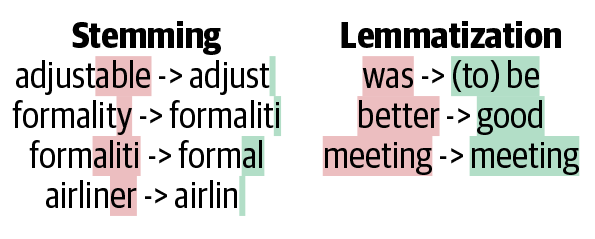
\includegraphics[width=0.65\textwidth]{capitulo3/figuras/nlp2.png}
	\caption{Diferencias entre la derivación y lematizacion
		\\\textit{Fuente: Extraído de} \protect\cite[p. 54]{vajjala2020practical}}
	\label{fig:nlp2}
\end{figure}
	
	\item Eliminar caracteres no alfabéticos: Eliminar signos de puntuación, números, símbolos, direcciones web y otros caracteres no alfabéticos simplifica el texto para un análisis y procesamiento más sencillo. La eliminación de estos caracteres innecesarios reduce el ruido en el análisis, mejorando la calidad y precisión de los modelos. Para esta tarea específica, el uso de expresiones regulares en funciones es altamente recomendado, ya que el tratamiento de cada conjunto de datos es diferente, debido a que cada uno tiene sus propias particularidades.
	
	\item Minúsculas: Transformar todo el texto en minúsculas es importante para unificar el tratamiento de palabras. Esta normalización del texto asegura una representación uniforme de las palabras bajo un mismo sistema de codificación, evitando que el modelo distinga entre palabras escritas con mayúsculas o minúsculas. Además, reduce la carga computacional al disminuir la cantidad de palabras distintas que el modelo necesita procesar, lo que mejora la eficiencia del análisis.

	\item Eliminar stopwords: Eliminar palabras comunes (stopwords) que no agregan valor al análisis, como ``el'', ``la'', ``y'', etc. Estas palabras son frecuentes en el lenguaje y aparecen en casi todos los textos. Al eliminarlas, se reduce la dimensionalidad del espacio de características y hace que el enfoque se centre en palabras clave y términos más significativos para el análisis.
	
	\item Corrección de errores ortográficos: Identificar y corregir errores ortográficos puede mejorar la precisión del análisis. Su efectividad puede variar dependiendo del contexto y del propósito del análisis. En entornos donde la precisión en la escritura es esencial, como la traducción automática o el análisis de sentimientos, corregir los errores ortográficos puede ser beneficioso. En ciertos casos, especialmente en análisis de texto informal o en redes sociales, conservar los errores ortográficos puede ser importante para capturar el tono o el estilo del texto original.
	
	\item Tratamiento de emojis: Los emojis son representaciones visuales cuya presencia puede ser crucial para comprender el tono, la intención o las emociones expresadas en un texto. En algunos casos, es útil eliminar los emojis del texto si no aportan información relevante para la tarea de procesamiento o análisis. En otros casos los emojis pueden mapearse a palabras o frases que describan su significado o intención. Por ejemplo, un emoji sonriente podría ser mapeado a la palabra ``feliz'' o ``contento'', mientras que un emoji de tristeza podría mapearse a ``triste'' o ``decepcionado''. 
Si no se decide hacer ninguno de los pasos anteriores y se considera mantenerlos en su estado original es importante convertir estos caracteres especiales a una representación más simple para su tratamiento.``Para analizar dichos símbolos no textuales y caracteres especiales, utilizamos la normalización Unicode. Esto significa que el texto que vemos debe convertirse en alguna forma de representación binaria para almacenarlo en una computadora. Este proceso se conoce como codificación de texto. Ignorar los problemas de codificación puede provocar errores de procesamiento en el futuro.''\cite[p. 45]{vajjala2020practical}.

\end{itemize}

El preprocesamiento de texto es esencial para preparar los datos de texto para su análisis, ayudando a eliminar ruido, reducir la dimensionalidad y mejorar la calidad de los datos, antes de aplicarlo a modelos de aprendizaje automático en tareas de NLP. También es importante mencionar que cada uno de los pasos de tratamiento de texto ya detallados no son obligatorios en su aplicación, que aplicar, en qué momento u orden depende solamente de lo que le convenga a la tarea que se quiere realizar 
	
	
	

\subsection{Ingeniería de características}
Si bien representar características es común en todo proyecto de ML, hacerlo con texto suele ser más complejo que con otros tipos de datos. Consideremos ejemplos como imágenes: almacenamos imágenes como matrices de píxeles, cada uno representando la intensidad de un píxel en la imagen. Con videos, cada cuadro se convierte en una matriz. En cuanto al habla, registramos la amplitud de una onda sonora en intervalos de tiempo fijos. Sin embargo, representar matemáticamente texto después de haberlo dividido en alguna unidad léxica para luego deducir el significado de cada unidad, comprender la estructura gramatical, entender el contexto en el que aparece y finalmente gracias a estos datos discernir la semántica, no es tan fácil. Esta sección  se sumerge en múltiples esquemas para abordar esta complejidad, desde métodos simples hasta las últimas técnicas para representar texto, un desafío que ha sido un foco activo de investigación en las últimas décadas.

Los enfoques tomados para generar todo tipo de representaciones de texto que se detallaran a continuación, pueden ser: 

\begin{itemize}

	\item Similitud Distribucional : El significado de una palabra se extrae del contexto en el que aparece, no sólo del significado literal.

	\item Hipótesis Distribucional: Plantea que palabras en contextos similares tienen significados similares. La similitud entre palabras se basa en sus contextos de aparición.
	
	\item Representación Distribucional: Se basa en esquemas que utilizan vectores de alta dimensión para representar palabras, basados en una matriz de co-ocurrencia, misma que captura la co-ocurrencia de palabras y contextos.
	
	\item Representación Distribuida: Una versión más compacta y densa en vectores que la representación distribucional, para superar la ineficiencia computacional de los vectores altamente dimensionales.

	\item Incrustación: Es un mapeo entre el espacio vectorial de la representación distributiva y la representación distribuida para un conjunto de palabras.
	
	\item Semántica Vectorial: Métodos de PLN que buscan aprender representaciones de palabras basadas en propiedades distribucionales en grandes corpus.
\end{itemize}

En el campo del PNL, transformar texto en una forma numérica se llama representación de texto. A continuación se explorarán los distintos métodos para convertir texto en vectores numéricos, todos los que se encuentran clasificados como modelos espaciales vectoriales como one-hot, bag of words, bag of n-grams y TF-IDF  caen dentro del concepto de representación distribucional.

\begin{itemize}
\item Modelos espaciales vectoriales


Los modelos vectoriales espaciales son técnicas que representan las palabras como vectores en un espacio dimensional. Estos modelos tienen como objetivo capturar la semántica de las palabras al asignarles vectores en un espacio matemático, donde la proximidad entre los vectores refleja la similitud semántica entre las palabras. Un modelo de espacio vectorial  es un modelo algebraico simple, en su representación simple son vectores identificadores como un índice de números en un vocabulario de algún documento, párrafo o libro de texto. El modelo más común para medir esta similitud, es la similitud del coseno, ver ecuacion \ref{eq:e21}. Por ejemplo las frases: ``El cielo es azul'' y ``El sol es amarillo'', se pueden representar cada una como un vector numérico. Para calcular la similitud entre estos vectores, se puede utilizar  el coseno del ángulo entre ellos. Si estos vectores se alinean perfectamente, el coseno del ángulo es 1, lo que indica una similitud máxima. Si están en direcciones opuestas, el coseno es -1, lo que significa una similitud mínima.
\begin{equation} \label{eq:e21} 
	similarity = cos(\theta) = \frac{\mathbf{A} \cdot \mathbf{B}}{\left \|  \mathbf{A} \right \|_2\cdot \left \|  \mathbf{B} \right \|_2}=\frac{\displaystyle\sum_{i=1}^{n}A_iB_i}{\sqrt{\displaystyle\sum_{i=1}^{n}A_i^2}\sqrt{\displaystyle\sum_{i=1}^{n}B_i^2}}
\end{equation}


$A = $  Algun vector.\\
$B = $  Algun vector.\\
$\mathbf{A} \cdot \mathbf{B} =$ Es el producto punto entre los vectores $A$ y $B$.\\
$\left \|  \mathbf{A} \right \|_2\cdot \left \|  \mathbf{B} \right \|_2 = $ Indica la norma euclidiana o la norma $L_2$. \\
$L_2$  de un vector = Se calcula sumando el cuadrado de cada componente del vector y luego tomando la raíz cuadrada del resultado. Que es equivalente a: 
$\left \|  \mathbf{A} \right \|_2 = \sqrt{A_1^2 + A_2^2 + \cdots + A_n^2} $.\\


La calidad de los vectores depende de cómo capturan las propiedades lingüísticas del texto. Diferentes enfoques, como el conteo de palabras o modelos de lenguaje pre-entrenados (word embeddings), producen representaciones de texto en forma de vectores con diferentes niveles de fidelidad y utilidad.

\begin{itemize}

	\item ONE HOT ENCODING: En One-Hot Encoding, cada palabra se representa mediante un vector binario donde todas las posiciones son cero excepto una, que corresponde al índice de la palabra en un vocabulario. Si hay un total de N palabras en el vocabulario, cada palabra se representa como un vector de longitud N con un único ``1'' en la posición que indica su índice en el vocabulario y ``0'' en todas las demás posiciones. Por ejemplo, si se tiene un vocabulario con las palabras: ``perro'', ``gato'', ``pájaro'' y ``muerde'', la representación One-Hot de cada una sería:
\begin{Center}
	perro → [1, 0, 0,0]\\
	gato → [0, 1, 0,0]\\
	pájaro → [0, 0, 1,0]\\
	muerde → [0, 0, 0, 1]\\
	
\end{Center}

Donde:

La oración ``perro muerde gato'' sería representada como: [   [1, 0 ,0 , 0]   [0, 0, 0, 1]   [0, 1, 0, 0]  ]


Este tipo de representación textual  es intuitiva y fácil de implementar pero, presenta limitaciones significativas. La relación directa entre el tamaño del vector one-hot y el tamaño del vocabulario provoca representaciones dispersas donde la mayoría de las entradas son ceros, lo que resulta en ineficiencia computacional y riesgo de sobreajuste. Además, esta representación no ofrece una longitud fija para el texto y trata las palabras como entidades aisladas, careciendo de la capacidad para capturar relaciones semánticas entre ellas. El desafío de manejar palabras fuera del vocabulario (Out Of Vocabulary), no se puede abordar directamente con esta representación, se requiere la expansión y reentrenamiento del modelo para incluir nuevas palabras.

	\item BAG OF WORDS: El modelo Bag of Words (BoW) es una técnica básica  para representar texto numéricamente. Primero  se construye un vocabulario a partir del corpus de documentos. El vocabulario se compone de todas las palabras únicas presentes en el corpus, y cada palabra se la enumera de manera única. Luego, se representa cada documento como un vector numérico. Para ello, se cuenta la frecuencia de cada palabra del vocabulario en cada documento. Por ejemplo: 
Dada las oraciones: \textit{``El gato está en la casa gato''} y \textit{``El perro está afuera''}

Se construye el diccionario: {El=1, gato=2, está=3, en=4, la=5, casa=6, perro=7, afuera=8}. Los IDs serán enteros únicos entre $\left | \text{V} \right |$, Donde $\left | \text{V} \right |$ representa el tamaño del vocabulario.

Se realiza la representación BoW:
\begin{center}[h!]
	\begin{tabular}{c c c c c c c c c c}
		& El & gato & está & en & la & casa & perro & afuera &  \\
		Frase 1: & 1 & 2 & 1 & 1 & 1 & 1 & 0 & 0 & ←Conteo frase 1\\
		Frase 2: & 1 & 0 & 1 & 0 & 0 & 0 & 1 & 1 & ←Conteo frase 2\\
		
	\end{tabular}
\end{center}


El enfoque de BoW trata el texto como una colección de palabras sin considerar el orden ni el contexto en el que aparecen. Supone que el contenido de un texto asociado a una categoría específica en un conjunto de datos está representado por un conjunto único de palabras. Si dos fragmentos de texto comparten la mayoría de sus palabras, se asume que pertenecen a la misma categoría o grupo, por esta razón se puede inferir la categoría o clase a la que ese texto puede pertenecer. Es importante resaltar que el enfoque BoW simplifica el texto a su esencia más básica: las palabras y su frecuencia, sin tomar en cuenta su secuencia o estructura gramatical.

	\item BAG OF N-GRAMS.- Es una técnica utilizada que extiende el concepto de Bag of Words (BoW) al considerar no solo palabras individuales, sino también secuencias contiguas de palabras llamadas n-gramas.``Capta cierta información de contexto y orden de palabras. Por tanto, el espacio vectorial resultante es capaz de capturar alguna similitud semántica. Los documentos que tienen los mismos n-gramas tendrán sus vectores más cerca entre sí en el espacio euclidiano en comparación con documentos con n-gramas completamente diferentes.''\cite[p. 90]{vajjala2020practical}. Un n-grama es una secuencia continua de ``n'' elementos, que pueden ser caracteres, palabras o algún tipo de token, a medida que n aumente, la dimensionalidad aumentará igual rápidamente. Por ejemplo:

Dadas las oraciones: ``El gato está durmiendo'' y ``El perro está comiendo''

Una representación bigrama de palabras es equivalente a:
[ ``El gato'', ``gato esta'', ``está durmiendo'', ``El perro'', ``perro esta'', ``está comiendo'' ]

La representación BoN constara de un vector de seis dimensiones para cada documento: ``El gato está durmiendo'' → [1,1,1,0,0,0], ``El perro está comiendo'' → [0,0,0,1,1,1 ].


Es importante recordar que al igual que Bag of Words, Bag of N-Grams (BoN) no ofrece una solución directa al problema de OOV (Out Of Vocabulary), es decir, no tiene un mecanismo incorporado para tratar con palabras que no estaban presentes durante el entrenamiento del modelo.


	\item TF-IDF.- A diferencia de las anteriores técnicas de representación de texto, Frecuencia de término-Frecuencia inversa de documentos (Term Frequency-Inverse Document Frequency) es una técnica que evalúa la importancia de una palabra en un documento dentro de un corpus o conjunto de documentos. Su formula general se divide en dos componentes que se explicaran detalladamente. Ver ecuación \ref{eq:e22}

\begin{equation} \label{eq:e22}
	\textrm{TF-IDF} = \textrm{TF} \times \textrm{IDF}
\end{equation}

TF (Frecuencia del término) mide la frecuencia con la que una palabra específica aparece en un documento en relación con el total de palabras en ese documento. Básicamente, es la cantidad de veces que una palabra aparece, dividida por el total de palabras en el documento como se muestra en la ecuacion \ref{eq:e23}. Si una palabra aparece muchas veces en un documento específico, y no aparece en los demás documentos, entonces se considera que la palabra es importante para ese documento específico.

\begin{equation} \label{eq:e23}
	\textrm{TF}(t,d)=\frac{(\textrm{Number of occurrences of term }t\textrm{ in document }d)}{(\textrm{Total number of terms in the document } d)}
\end{equation}

IDF (Frecuencia inversa de documentos) mide la importancia de una palabra a través de todo el conjunto de documentos. Esta métrica reduce el peso de palabras comunes que aparecen en muchos documentos y aumenta el peso de palabras raras que podrían ser más significativas para un documento específico. Es decir, si se considera que una palabra es importante para un documento, pero esta aparece constantemente en los demás documentos entonces disminuye su importancia. Se calcula tomando el logaritmo del inverso de la frecuencia de documentos que contienen el término, y se suma uno para evitar la división por cero si el término no está presente en el corpus.

\begin{equation} \label{eq:e24}
	\textrm{IDF}(t)=\frac{(\textrm{Total number of documents in the corpus})}{(\textrm{Number of documents with term } t \textrm{ in them})}
\end{equation}

Esta técnica de representación se aplica para cada palabra en cada documento y se  pueden usar los vectores obtenidos para calcular la similitud entre dos textos, usando alguna medida de similitud como la distancia euclidiana o la similitud del coseno.


\end{itemize}

\item Representaciones distribuidas

Las representaciones distribuidas de texto buscan capturar el significado de palabras, oraciones o frases considerando su proximidad textual, en un espacio vectorial. Estas representaciones, conocidas como embeddings, abordan los desafíos de dimensionalidad y contexto crucial durante el entrenamiento. Para lograrlo, emplean arquitecturas de redes neuronales que generan representaciones de baja dimensión y alta densidad para palabras y textos.

\begin{itemize}

	\item Word embeddings: Las incrustaciones de palabras (word embeddings) son representaciones vectoriales de palabras en un espacio dimensional, donde cada palabra se asigna a un vector denso. Estos vectores son diseñados de manera que palabras con significados similares están cercanas entre sí en este espacio vectorial, además sus representaciones vectoriales de texto tienen dimensiones bajas y densas en comparación con representaciones one-hot encoding, lo que permite una manipulación más eficiente. Los modelos  más populares pueden ser: Word2Vec, GloVe y FastText, uno de los mayores representantes de los modelos embeddings es Word2Vec, que en si mismo es un conjunto de modelos que fueron fundamentales en el campo del Procesamiento del Lenguaje Natural. Desarrollado por un equipo de investigadores de Google, liderado por Tomás Mikolov, en 2013, fue un avance crucial en la generación de representaciones vectoriales de palabras, basadas en modelos de redes neuronales, cuya idea central era capturar y representar la semántica de las palabras a través de sus contextos en un corpus de texto \cite{mikolov2013efficient}. 
	
	\item Hiperparametros de embeddings: Algunos hiperparámetros comunes al trabajar con embeddings en modelos como Word2vec, GloVe, fastText o incluso en modelos más avanzados incluyen:  La dimensión del embedding, la cual  determina la longitud de los vectores; la ventana de contexto, controla cuántas palabras vecinas se van a considerar y el tamaño del vocabulario, ya que algunos modelos de embeddings tienen un límite en el tamaño del vocabulario a usar. Ajustar estos y otros  hiperparámetros correctamente puede influir significativamente en la calidad y el rendimiento de los embeddings resultantes.``El ajuste de hiperparámetros juega un papel clave: cualquier método funcionará mal si se utilizan los hiperparámetros incorrectos'' \cite[p. 339]{eisenstein2018natural}.
	
	\item Word2Vec.- El modelo Word2Vec se destaca por su capacidad para generar incrustaciones vectoriales significativas y densas para palabras, lo que permite representar el significado semántico de las palabras en un espacio vectorial de dimensiones bajas (vectores de dimensiones 50-500 en vez de varios miles). Su eficiencia para la representación de palabras fue tal, que se observaron habilidades para resolver analogías y capturar relaciones de significado entre palabras como:  
	\begin{Center}
			$Rey - Hombre + Mujer \approx  Reina$.
	\end{Center}

	
Word2vec es un conjunto redes neuronales poco profundas que utilizan la similitud distributiva e hipótesis distributiva para aprender  el significado de las palabras ``El modelo Word2vec perfecciona los valores en $v_w$ al predecir $v_{w'}$, dados los vectores para las demás palabras en el contexto C.'' \cite[p. 95]{vajjala2020practical} .

Word2Vec funciona utilizando dos arquitecturas principales: Continuous Bag of Words (Cbow) y Skip-gram.

\begin{figure}[h!]
	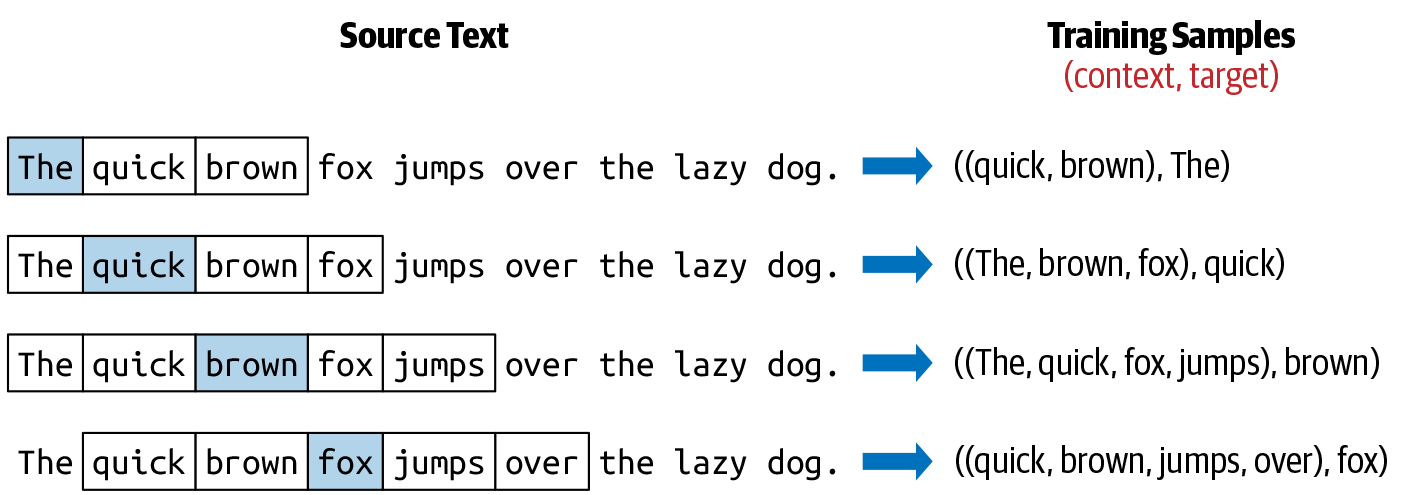
\includegraphics[width=0.65\textwidth]{capitulo3/figuras/nlp3.png}
	\caption{Preparando un conjunto de datos por CBOW
		\\\textit{Fuente: Extraído de} \protect\cite[p. 99]{vajjala2020practical}}
	\label{fig:nlp3}
\end{figure}

Cbow: Predice la palabra objetivo basándose en un contexto de palabras adyacentes, tomará cada palabra del corpus como palabra objetivo e intentará predecir la palabra objetivo a partir de sus palabras de contexto correspondientes. Por ejemplo, teniendo un tamaño de contexto dos (k=2), el  tamaño de la ventana deslizante será igual a 2k +1 donde uno representará  a la ventana central. Ver Figura \ref{fig:nlp3}



\begin{figure}[h!]
	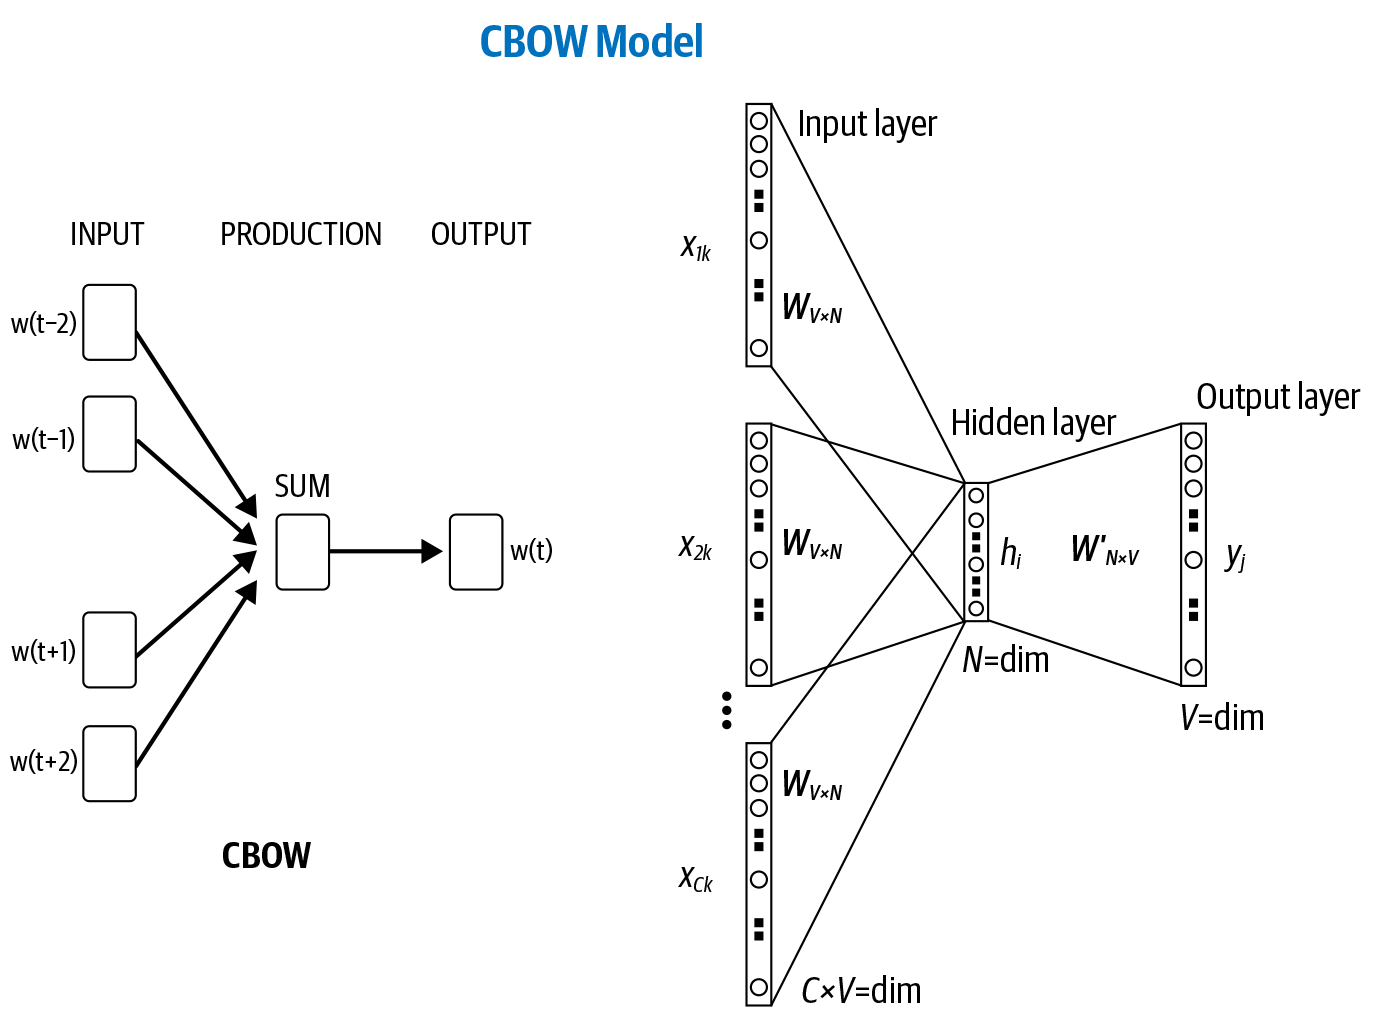
\includegraphics[width=0.65\textwidth]{capitulo3/figuras/nlp4.png}
	\caption{Modelo CBOW
		\\\textit{Fuente: Extraído de} \protect\cite[p. 100]{vajjala2020practical}}
	\label{fig:nlp4}
\end{figure}

El modelo Cbow utiliza una red neuronal poco profunda para aprender incrustaciones vectoriales de palabras. Esta red tiene una capa oculta y su objetivo es aprender una matriz de incrustación de palabras (definida como $E_{ \left | \textrm{V}  \right |\: \textrm{x} \: \textrm{d}}$,  donde $\left | \textrm{V}  \right | = $ tamaño del vocabulario, d= dimensión de incrustación)  a partir de un vocabulario (v)  dado inicialmente  \ref{fig:nlp4}. La matriz de incrustación se inicia de forma aleatoria. Posteriormente  la red selecciona vectores de las palabras del contexto de la matriz y los combina para generar un vector (d), que luego se multiplica con otra matriz ${E}'_{ \textrm{d} \: \textrm{x}  \:\left | \textrm{V}  \right | }$ en la siguiente capa. Esto da como resultado un vector de una dimensión por el tamaño del vocabulario ( $1 \times \left | \textrm{V}  \right |$) que funge como entrada para una función softmax para obtener la distribución de probabilidad en el espacio de vocabulario. Al final del entrenamiento, la matriz de incrustación $E$ y $E'$ obtenida se actualizan después de comparar la distribución aprendida con la etiqueta (palabra objetivo) mediante retropropagación.

\begin{figure}[h!]
	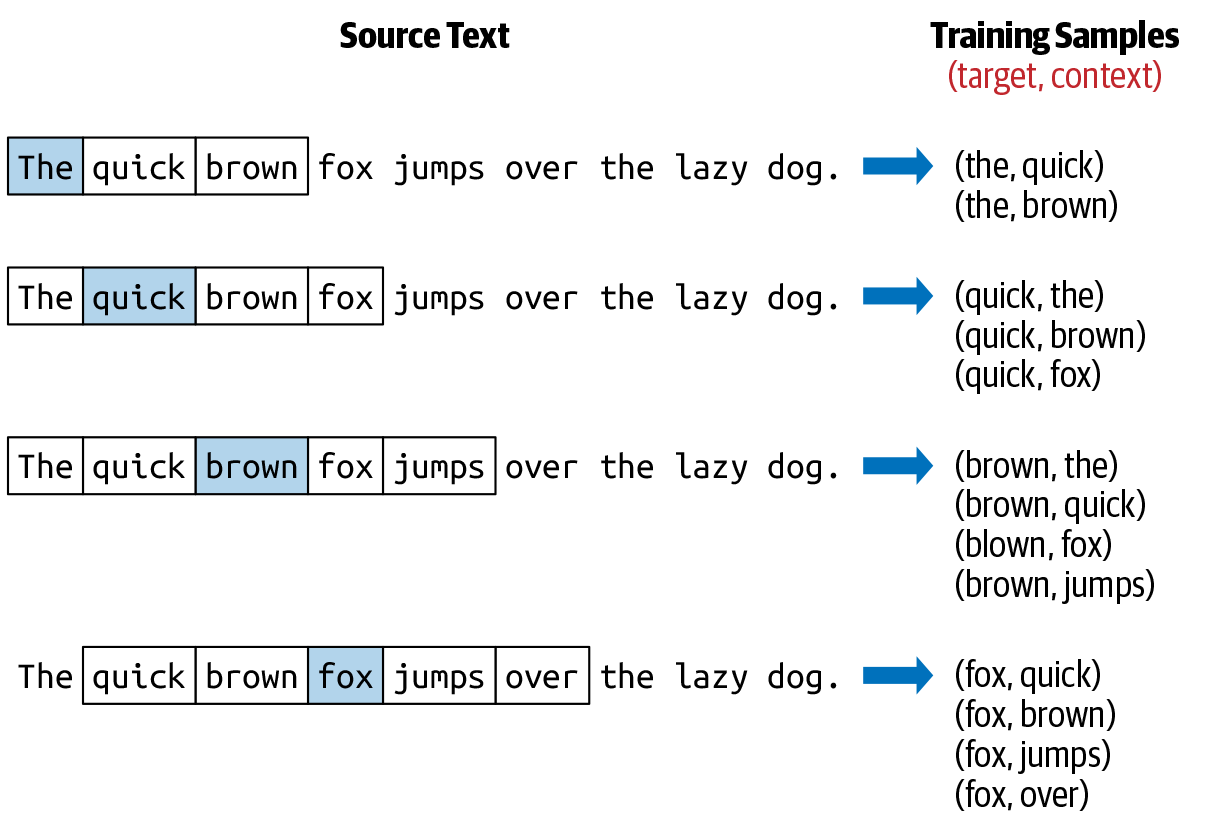
\includegraphics[width=0.6\textwidth]{capitulo3/figuras/nlp5.png}
	\caption{Preparando un conjunto de datos por SkipGram
		\\\textit{Fuente: Extraído de} \protect\cite[p. 101]{vajjala2020practical}}
	\label{fig:nlp5}
\end{figure}

Skip-gram: Predice las palabras del contexto a partir de la palabra central. Toma una palabra de entrada y predice las palabras que podrían aparecer en su contexto.``El conjunto de datos para entrenar un SkipGram se prepara de la siguiente manera: ejecutamos una ventana deslizante de tamaño 2k+1 sobre el corpus de texto para obtener el conjunto de 2k+1 palabras que están bajo consideración. La palabra central en la ventana es la X, y las k palabras a cada lado de la palabra central son Y'' \cite[p. 101]{vajjala2020practical}. Al igual que el modelo cbow, k representara el número de palabras, pero en este caso serán las que se deben predecir ver Figura \ref{fig:nlp5}



\begin{figure}[h!]
	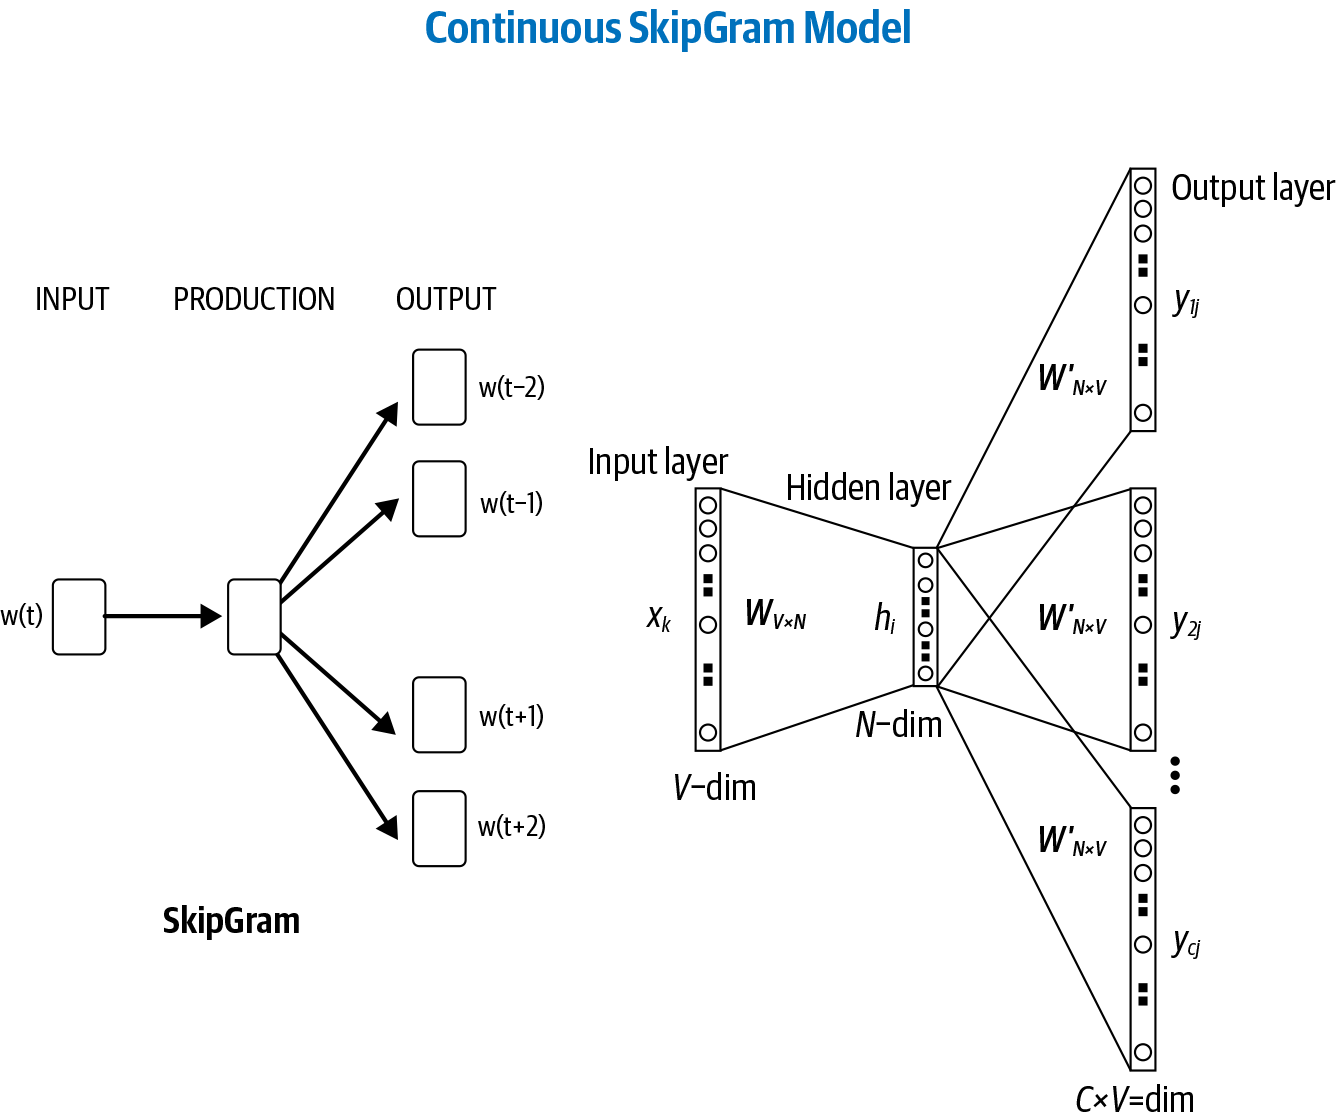
\includegraphics[width=0.65\textwidth]{capitulo3/figuras/nlp6.png}
	\caption{Modelo SkipGram
		\\\textit{Fuente: Extraído de} \protect\cite[p. 102]{vajjala2020practical}}
	\label{fig:nlp6}
\end{figure}

En el modelo SkipGram, se emplea una red similar a la usada en CBOW. En la capa de entrada, se toma el índice de la palabra objetivo para acceder a su vector correspondiente en la matriz de incrustación $E_{ \left | \textrm{V}  \right |\: \textrm{x} \: \textrm{d}}$,  donde $\left | \textrm{V}  \right | = $  , estos vectores se combinan y forman un nuevo vector que se multiplica por otra matriz ${E}'_{ \textrm{d} \: \textrm{x}  \:\left | \textrm{V}  \right | }$  para obtener un vector unidimensional de probabilidad en el espacio del vocabulario. La comparación entre esta distribución y la etiqueta se utiliza para actualizar las matrices de incrustación a través de la retropropagación. Al finalizar el entrenamiento, la matriz de incrustación obtenida (denotada como $E_{ \left | \textrm{V}  \right |\: \textrm{x} \: \textrm{d}}$) representara las palabras del vocabulario en vectores de baja dimensión.Ver Figura \ref{fig:nlp6}

	\item Word embeddings pre entrenados:  Son representaciones vectoriales de palabras generadas mediante modelos de lenguaje que han sido entrenados previamente con grandes cantidades de texto. Los embeddings pre entrenados más populares como wor2vec, glove y fastext que ya se mencionaron están disponibles para varias dimensiones como d = 25, 50, 100, 200, 300, 600. De igual forma, en muchas ocasiones, los investigadores comparten embeddings de palabras ya entrenados para ser utilizados libremente en proyectos académicos o comerciales. Cuando se opta por utilizar embeddings previamente entrenados, se tiene dos enfoques principales:
	
Estático: Implica emplear los embeddings tal como están, sin modificarlos. Esto es ideal si los embeddings se ajustan bien al problema y ofrecen buenos resultados.

Actualizado: Se basa en utilizar los embeddings pre entrenados para inicializar el modelo, pero se permite que se actualicen durante el entrenamiento. Esta opción puede ser beneficiosa si se busca integrar y mejorar el modelo en una tarea específica.

Si en estos modelos pre-entrenados no existieran representaciones vectoriales de palabras importantes para la tarea en cuestión, dependiendo de la librería en uso, se pueden reentrenar. 

Para decidir si reentrenar modelos previamente entrenados, una buena regla general es calcular la superposición de vocabulario. Si la superposición entre el vocabulario de nuestro dominio personalizado y el de las incrustaciones de palabras previamente entrenadas es superior al 80\%, las incrustaciones de palabras pre-entrenadas tienden a dar buenos resultados en la clasificación de texto.``Si la superposición entre el vocabulario del corpus y el vocabulario incorporado es inferior al 80\%, es poco probable que veamos un buen desempeño de nuestro modelo de PNL.''\cite[p. 104]{vajjala2020practical}.

	\item Oov y embeddings.- Abordar el problema de las palabras fuera del vocabulario en los modelos de embeddings es todo un desafío, ya que  las palabras fuera del vocabulario no tienen representaciones predefinidas, lo que dificulta su procesamiento y comprensión. Si se quiere rehusar embeddings pre entrenados para saltarse la difícil tarea de entrenar un embedding que requiere de miles y miles de datos para obtener una representación más o menos buena se debe considerar que las representaciones que se encuentren son suficientes y se adaptan al problema, o qué nuevas palabras deben añadirse. Para incorporar palabras nuevas a modelos que ya han sido entrenados, hay algunas estrategias que se pueden utilizar como:

El entrenamiento incremental: implica volver a ejecutar el algoritmo de entrenamiento con el corpus actualizado, que contiene las nuevas palabras. Esto puede ser costoso computacionalmente, en especial si el corpus es grande. 

Inicialización de vectores: Se pueden agregar palabras nuevas asignándoles vectores aleatorios o utilizando algún otro método de inicialización específico.``Una forma de lidiar con el problema OOV para incrustaciones de palabras es crear vectores que se inicializan aleatoriamente, donde cada componente está entre –0,25 y +0,25, y continuar usando estos vectores en toda la aplicación''\cite[p. 105]{vajjala2020practical}.

Sub-palabras: Modelos como FastText abordan el problema de OOV representando las palabras a través de sus constituyentes de caracteres, es decir, descomponiendo las palabras en n-gramas de caracteres (secuencias de caracteres de longitud n. En lugar de solo aprender incrustaciones de palabras completas, también aprende incrustaciones de n-gramas de caracteres. La representación de una palabra se construye agregando las incrustaciones de sus n-gramas de caracteres constituyentes.

Textos Completos:  Otro enfoque para lidiar con el problema OOV, es Doc2Vec. Es una técnica de aprendizaje no supervisado que genera representaciones vectoriales densas para documentos, lo que permite medir la similitud y realizar operaciones semánticas en documentos completos. ``es similar a Word2vec en cuanto a su arquitectura general, excepto que, además de los vectores de palabras, también aprende un ``vector de párrafo'' que representa el texto completo (es decir, con palabras en contexto).''\cite[p.106]{vajjala2020practical}. El vector de párrafo representa un texto completo (un párrafo, una oración o incluso un documento entero). 

Las redes neuronales superficiales utilizadas para aprender las incrustaciones de Doc2vec son parecidas a CBOW y SkipGram de Word2vec, el primer modelo se denomina memoria distribuida (DM) donde se integra tanto la información del contexto de palabras como la representación del documento completo para predecir la palabra objetivo. Esto permite que el modelo capture no solo el significado de las palabras individuales en un contexto, sino también la esencia general del documento en el que aparecen esas palabras. El segundo modelo se denomina bolsa de palabras distribuida (DBOW) este modelo omite la predicción de palabras y se centra únicamente en predecir el siguiente documento basándose solo en el vector de documento.
	
	\item Consideraciones.- A continuación se detallaran consideraciones importantes que tomar respecto al uso de embeddings pre entrenados:\\
Sesgo.-  Las representaciones de texto, como embeddings o vectores que capturan el significado de las palabras o textos, están influenciadas por los datos con los que se entrenan. Estos sesgos pueden tener impactos significativos en el rendimiento de los modelos que dependen de estas representaciones.\\

Exigencia computacional.- Los embeddings pre entrenados suelen ser archivos grandes, a menudo varios gigabytes. Este tamaño puede causar dificultades en el rendimiento si no se aborda adecuadamente. Por ejemplo, el modelo Word2vec requiere aproximadamente 4,5 GB de memoria RAM, lo que puede ser un desafío en ciertos escenarios.
\\
Representar necesidades.- Existen necesidades lingüísticas y de aplicación que van más allá de lo que las técnicas de embeddings pueden capturar actualmente. Por ejemplo, la detección de sarcasmo es una tarea que requiere matices y sutilezas que aún no son bien representadas o entendidas completamente mediante técnicas de embeddings.\\

Estado del arte.- La representación neuronal del texto es un área en constante evolución en el campo del procesamiento del lenguaje natural (PNL), con avances rápidos en el estado del arte. Aunque nuevos modelos suelen generar entusiasmo, es importante considerar aspectos prácticos, usar modelos nuevos no siempre será la mejor opción, es importante considerar que también se pueden tener buenos resultados con modelos de embeddings básicos, que además no requieren de mucha capacidad computacional. 

\end{itemize}
\end{itemize}




\subsection{Modelado}
En esta sección, se explorará cómo transformar los datos recopilados en una solución efectiva para un proyecto de procesamiento de lenguaje natural. Con datos iniciales limitados, se comienza con métodos sencillos y reglas básicas, incrementando gradualmente la complejidad a medida que se obtienen más datos y una mejor comprensión del problema. Algunos enfoques que pueden ayudar en la construcción de un modelo efectivo son los siguientes:

\begin{itemize}

\item Construcción de heurísticas: Al principio las heurísticas y las expresiones regulares pueden ser herramientas clave para abordar tareas específicas en las primeras etapas del desarrollo del modelo, permitiendo la extracción de información relevante incluso sin contar con grandes volúmenes de datos de entrenamiento. proporcionando una base sólida mientras se recopilan suficientes datos para aplicar técnicas más avanzadas de aprendizaje automático. Por ejemplo en la clasificación de texto ofensivo si se identifica ciertas palabras clave como ofensivas se pueden clasificar directamente como ofensivas en lugar de enviarlas al modelo, o en cambio, se pueden crear características a partir de estas heurísticas para entrenar el modelo.

\item Ensamble y Apilamiento: En el ámbito del aprendizaje automático, una práctica común es utilizar una colección de modelos en lugar de depender de un solo modelo para abordar diferentes aspectos del problema de predicción. Existen dos enfoques principales para lograr esto. El primero es el apilamiento de modelos, donde la salida de un modelo se utiliza como entrada para otro, siguiendo una secuencia hasta obtener una predicción final. El segundo enfoque es el ensamble de modelos, que consiste en combinar las predicciones de múltiples modelos y realizar una predicción final conjunta. El uso de múltiples modelos para la resolución de algún problema puede mejorar de manera significativa una predicción, es un camino que se debe tomar en cuenta.

\item Mejor Ingeniería de Características: Un buen proceso de ingeniería de características puede mejorar significativamente el rendimiento del modelo. Cuando hay muchas características disponibles, la selección de las más relevantes ayuda a optimizar el modelo.

\item Aprendizaje por transferencia: El aprendizaje por transferencia permite que un modelo nuevo adquiera conocimientos de un modelo grande y bien entrenado, lo que mejora su comprensión del lenguaje y del problema específico. Esto es similar a cómo un profesor transmite conocimientos a un estudiante. Esta técnica facilita las tareas posteriores, especialmente cuando se dispone de un conjunto de datos limitado, y suele ofrecer mejores resultados que comenzar a entrenar un modelo desde cero con una inicialización aleatoria.

\item Reaplicación de Heurísticas: Dado que los modelos de aprendizaje automático no son perfectos y cometen errores, es posible revisar estos errores al final del proceso de modelado para identificar patrones comunes y corregirlos mediante heurísticas. Además, se puede utilizar conocimiento específico del dominio, que no se captura automáticamente en los datos, para mejorar las predicciones del modelo.

\end{itemize}



\subsection{Evaluación}
Se puede evaluar un modelo de manera intrínseca y extrínseca. A continuación, se detalla la definición de ambos términos en este contexto.

\begin{itemize}

\item Evaluación intrínseca:  En la evaluación intrínseca de sistemas de procesamiento de lenguaje natural, se emplean conjuntos de prueba con etiquetas proporcionadas por humanos, que pueden ser binarias, de una a dos palabras o textos extensos. Se compara la salida del modelo de PLN con estas etiquetas para calcular métricas que reflejen la precisión del modelo en diferentes tareas. Esta evaluación puede automatizarse en la mayoría de las tareas de PLN, aunque hay casos como la traducción automática o la sumarización donde la evaluación automatizada puede ser subjetiva y difícil de implementar. Para las clasificaciones, la matriz de confusión es una herramienta visual comúnmente utilizada que permite la comparación entre la salida predicha y la salida real, facilitando el cálculo de métricas como precisión, recall, puntaje F1 y exactitud, fundamentales para medir el desempeño del modelo.


\item Evaluación extrínseca: La evaluación extrínseca se enfoca en medir cómo el modelo se desempeña en el objetivo final de un proyecto industrial de inteligencia artificial, el cual busca resolver problemas empresariales específicos. Aunque la evaluación extrínseca es crucial, se realiza también la evaluación intrínseca porque esta última puede ser realizada internamente por el equipo de IA, antes de involucrar a partes interesadas externas como usuarios finales. Esto ayuda a reducir costos, ya que la evaluación extrínseca puede ser más costosa. Los malos resultados en la evaluación intrínseca generalmente indican malos resultados en la evaluación extrínseca, pero el buen desempeño intrínseco no siempre garantiza buenos resultados extrínsecos. Las razones de un rendimiento deficiente en la evaluación extrínseca pueden incluir métricas inapropiadas, falta de datos adecuados o expectativas erróneas.

\end{itemize}

\subsection{Despliegue del modelo}
Un módulo de procesamiento de lenguaje natural se implementa típicamente como un servicio web que recibe texto como entrada y devuelve la categoría del texto como salida. En aplicaciones prácticas, el módulo suele formar parte de un sistema más grande y debe desplegarse en un entorno de producción integrado, garantizando que las canalizaciones de datos de entrada y salida estén optimizadas y que el módulo sea capaz de manejar cargas elevadas de manera eficiente.
\subsection{Monitoreo y actualización}
Antes del despliegue final de cualquier proyecto de ingeniería de software, es fundamental realizar pruebas exhaustivas del software y monitorear continuamente el rendimiento del modelo una vez desplegado. En proyectos y modelos de procesamiento de lenguaje natural, el monitoreo debe ser especialmente cuidadoso para garantizar que las salidas diarias del modelo sean coherentes y útiles. Si el modelo se entrena automáticamente con frecuencia, es crucial asegurar que su comportamiento sea adecuado, algo que se facilita mediante un panel de rendimiento que muestra parámetros y métricas clave del modelo. Además, una vez que el modelo está en producción y se comienzan a recopilar nuevos datos, se realiza una iteración continua del modelo con estos datos para mantener sus predicciones actualizadas.
\section{DEEP LEARNING PARA LA CLASIFICACIÓN DE TEXTO}
Al trabajar con redes neuronales, se requiere un procesamiento adicional de los vectores de entrada para adaptarlos a las capas de entrada de la red neuronal. Estos pasos describen la preparación de datos para usarlos como entrada en una arquitectura de red neuronal en el contexto del procesamiento de lenguaje natural. Si bien estos pasos ya se mencionaron anteriormente es importante resaltarlos ya que son fundamentales para preparar datos textuales, debido a que transforman los textos en representaciones numéricas adecuadas que pueden ser entendidas y procesadas por la red neuronal.

\begin{itemize}

	\item Tokenización: Consiste en dividir los textos en unidades más pequeñas, como palabras o subpalabras (tokens).
	
	\item Conversión a vectores de índices de palabras: Asigna un número único a cada palabra o token del texto.

	\item Relleno de secuencias de texto para tener la misma longitud: En muchos modelos de redes neuronales, todas las secuencias deben tener la misma longitud. Si las secuencias de texto tienen longitudes diferentes, se pueden rellenar con valores específicos (como 0) para que todas tengan la misma longitud. Por ejemplo, si el máximo de palabras permitidas es 100 y un texto tiene 80 palabras, se pueden agregar 20 valores de relleno al final.
	
	\item Asignación de índices de palabras: Cada índice de palabra (número único) se asigna a un vector de incrustación correspondiente. Se multiplican los vectores índice de palabras con la matriz de incrustación para obtener vectores de incrustación asociados a cada palabra en el texto.
	
	\item Uso del resultado como entrada: Los vectores de incrustación resultantes, que representan las palabras de los textos y están listos para ser procesados por la red neuronal, se utilizan como la entrada para la arquitectura de la red neuronal.

\end{itemize}

\section{LAS REDES SOCIALES Y EL PLN}
El texto extraído de las redes sociales presenta desafíos y problemas específicos debido a la naturaleza única de estos datos. Algunos de los problemas comunes son:

\begin{itemize}

	\item Ruido y calidad del texto: Los datos de redes sociales suelen contener errores ortográficos, abreviaturas desenfrenadas, emojis, jerga, sarcasmo, uso  de mayúsculas inconsistentes, repetición de caracteres y lenguaje informal. Las conversaciones en especial en las redes sociales no siguen ninguna gramática, además de tener contenido irrelevante como propaganda.``Las publicaciones en las redes sociales están llenas de spam, anuncios, contenido promocionado y todo tipo de contenido no solicitado, irrelevante o que distrae''\cite[p. 283]{vajjala2020practical}. Esto puede dificultar la comprensión y el análisis del texto, ya que requiere un preprocesamiento más cuidadoso para lidiar con estas peculiaridades.
	
	\item Variabilidad lingüística y diversidad de idiomas: Las redes sociales son utilizadas a nivel mundial, lo que significa que los datos provienen de una amplia gama de idiomas y dialectos. Esta variabilidad lingüística agrega complejidad al procesamiento de texto y a la construcción de modelos que funcionen adecuadamente en diferentes idiomas.
	
	\item Vocabulario en constante evolución.- Las redes sociales son semilleros para la creación de nuevos términos y modismos que pueden volverse virales rápidamente. ``cuando se trata del lenguaje social, el vocabulario aumenta a un ritmo muy rápido. Cada día aparecen nuevas palabras. Esto significa que cualquier sistema de PNL que procese SMTD ve muchas palabras nuevas que no formaban parte del vocabulario de los datos de entrenamiento''. \cite[p. 281]{vajjala2020practical}. Los modelos de PLN deben ser capaces de adaptarse rápidamente a estos cambios en el vocabulario. La actualización constante de estos modelos para capturar nuevos términos y usos del lenguaje se vuelve esencial para mantener la eficacia en la comprensión de texto en entornos de redes sociales.
	
	\item Ambigüedad y contexto: Los mensajes en redes sociales pueden carecer de contexto, lo que lleva a ambigüedad en el significado. La falta de contexto puede dificultar la interpretación precisa del texto, especialmente en el caso de ironías, dobles sentidos o mensajes sarcásticos.	
\end{itemize}

\begin{figure}
	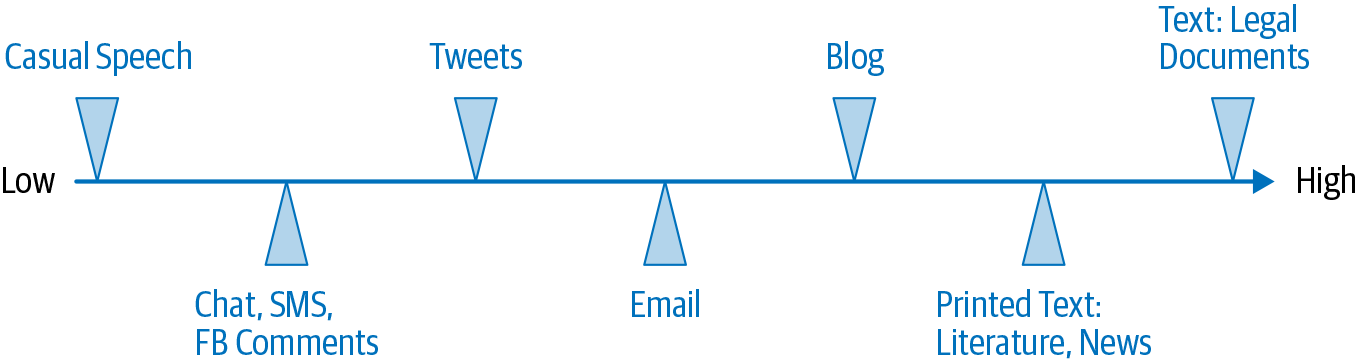
\includegraphics[width=0.65\textwidth]{capitulo3/figuras/nlp7.png}
	\caption{Espectro de formalismo en textos según sus fuentes}
	\floatfoot{Fuente: Practical natural language processing: A comprehensive guide to building real-world NLP systems \cite[p. 283]{vajjala2020practical} }
	\label{fig:nlp7}
\end{figure}

Los datos textuales provenientes de redes sociales tienden a ser considerablemente más informales en comparación con textos provenientes de blogs, libros, artículos de noticias o documentos legales.

 La Figura \ref{fig:nlp7} ilustra el espectro de formalidad en los datos de texto, ubicando diferentes fuentes de datos textuales dentro de este espectro.



Es esencial comprender la distinción entre el procesamiento de texto formal y el extremadamente informal, como el que se encuentra en las redes sociales. La labor de limpieza en este último caso debe ser más minuciosa: implica revisar exhaustivamente el texto para identificar qué aspectos se deben limpiar y qué herramientas o funciones adicionales se deben implementar para eliminar las particularidades presentes. Se requiere una cantidad significativa de tiempo y esfuerzo humano para dejar el texto en condiciones utilizables para las fases posteriores. Se hace un énfasis al esfuerzo humano debido a que el uso de herramientas existentes para el texto de redes sociales probablemente no den resultados tan satisfactorios. Estas herramientas están diseñadas para operar de manera más general y no específicamente adaptadas para manejar las características únicas que se pueden encontrar en este tipo de texto tan dinámico.



%\section{CONJUNTOS DE DATOS RELACIONADOS CON EL LENGUAJE OFENSIVO}
%Existen diversos conjuntos de datos relacionados con el lenguaje ofensivo extraídos de distintas redes o plataformas sociales. Muchos de estos conjuntos se encuentran mayormente en inglés, como el conjunto de datos ``Hate Speech and Offensive Language'' disponible públicamente en Kaggle, mismo que contiene mensajes recopilados de la red social Twitter. Este conjunto de datos alberga 2,458,155 tweets publicados por usuarios que expresan odio.

Encontrar conjuntos de datos en español es un desafío, uno de los pocos conjuntos disponibles es ``Offendes'', enfocado en influencers jóvenes de plataformas sociales como Twitter, Instagram y YouTube. Este corpus recopilado está compuesto por comentarios en español etiquetados manualmente como: ofensivos, dirigidos a un individuo específico (OFP); ofensivos, dirigidos a grupos basados en etnia, género, orientación sexual, ideología política, creencia religiosa u otras características comunes (OFG); no ofensivos pero con lenguaje grosero (NOE), y finalmente, no ofensivos (NO). El conjunto de datos público de Offendes contiene 30,416 muestras seleccionadas el total usado en la tarea ``MeOffendes'' en el IberLEF 2021. El IberLEF (Iberian Languages Evaluation Forum) es un espacio de evaluación que se enfoca en los desafíos y avances del procesamiento de lenguaje natural para las lenguas ibéricas, incluyendo el español, portugués y otras lenguas regionales como el catalán y el gallego.

Offendes se divide en tres subconjuntos: entrenamiento con 16,710 muestras, desarrollo con 100 muestras y prueba con 13,606. Para un detalle más específico sobre la cantidad de datos etiquetados, ver la tabla \ref{tbl:13}. Este conjunto de datos se usará con el fin de ayudar en el etiquetado de los datos recopilados y además para tener más variabilidad en los datos.

\begin{table}[!ht]
	\centering
	\begin{tabular}{|c|c|c|c|}
		\hline
		\textbf{Label} & \textbf{Training} & \textbf{Development} & \textbf{Test} \\ \hline
		NO & 13212 & 64 & 9651 \\ 
		NOE & 1235 & 22 & 2340 \\ 
		OFP & 2051 & 10 & 1404 \\ 
		OFG & 212 & 4 & 211 \\ \hline
		\textbf{Total} & 16710 & 100 & 13606 \\ \hline
	\end{tabular}
	\caption{Detalle distribucion categorias OffendES}
	\label{tbl:13}
\end{table}


%\section{CREACIÓN DEL CONJUNTO DE DATOS RELACIONADO CON EL LENGUAJE OFENSIVO EN EL CONTEXTO BOLIVIANO}
%El conjunto de datos utilizado en este proyecto fue recopilado exclusivamente de dos plataformas de redes sociales: Facebook y WhatsApp. Se extrajo una cantidad significativa de muestras, las cuales fueron sometidas a un exhaustivo proceso de preprocesamiento y análisis. Durante este proceso, se realizaron diversas operaciones de limpieza para garantizar la calidad y relevancia de los datos.

Como resultado de estas operaciones de limpieza, las cifras originales de muestras variaron. A continuación, se presentan dos tablas que resumen este proceso: La tabla 1 muestra la cantidad inicial de comentarios extraídos, incluyendo aquellos que contenían enlaces, duplicados y contenido no relevante, entre otros aspectos. La tabla presenta la cantidad final de comentarios considerados útiles después de haber sido sometidos al proceso de limpieza. Se eliminaron duplicados y se aplicaron filtros para garantizar la calidad y relevancia de los datos.

tabla 1
-------------------------------------------------------------
cifras originales de comentarios extraidos:
Conjunto de datos
Santa Cruz   16380
La Paz          15861
Cbba             38913
WhatsApp     20826
total comentarios 91980
cifras finales despues de la limpieza
---------------------------------------------------------------

tabla 2
-----------------------------------------------------------
Conjunto de datos
Santa Cruz  14385
La Paz 14229
Cbba 35863
WhatApp 14501
total comentarios 78978
-----------------------------------------------------------

Los comentarios cuyas cifras han sido presentadas en las tablas anteriores fueron cuidadosamente seleccionados para reflejar la diversidad y riqueza de la comunicación en cada uno de los nueve departamentos de Bolivia. Estos departamentos están divididos en tres regiones distintas: el altiplano, que incluye La Paz, Oruro y Potosí; los valles, que abarcan Chuquisaca, Cochabamba y Tarija; y los llanos, que comprenden Santa Cruz, Pando y Beni.

Esta selección se llevó a cabo considerando variantes existentes en el uso del idioma español en cada región del país. Además, se decidió focalizar en un departamento específico de cada zona debido a la distribución demográfica característica de cada uno. Por ejemplo, los departamentos de Santa Cruz, La Paz y Cochabamba albergan la mayor cantidad de habitantes en sus respectivas regiones, lo que los convierte en representantes significativos de la diversidad lingüística y cultural de Bolivia.



%\subsection{Palabras clave y elección de comentarios}
%A continuación se brindarán detalles sobre la recolección de comentarios en las redes sociales de facebook y whatsapp.

\textbf{Facebook}

Todos los comentarios de la red social Facebook fueron extraídos de forma manual, empleando palabras o frases clave durante la búsqueda de las publicaciones correspondientes. Esta práctica se llevó a cabo debido a la falta de un control sobre la ubicación geográfica de las publicaciones en Facebook. A continuación se presentan las palabras clave seleccionadas:
\begin{itemize}
	\item racista /racismo
	\item sexista/sexismo
	\item homosexual/homofobia/homofobico
	\item lenguaje ofensivo/lenguaje de odio 
	\item discriminar/discriminacion
	\item machista/machismo
	\item violento/violencia
	\item feminista/feminismo  
\end{itemize}
y los nombres de las ciudades de Bolivia que se usaron conjuntamente con cada uno de las palabras clave en la búsqueda para encontrar comentarios ofensivos en la red social facebook:
\begin{itemize}
	\item Cochabamba
	\item Santa Cruz
	\item La Paz
	
\end{itemize}

Además de utilizar palabras clave para identificar publicaciones relevantes para este proyecto, también se llevó a cabo la selección de perfiles de autoridades políticas, medios de información y medios de comunicación en Bolivia. Esto se hizo con la comprensión de que los temas políticos y los hechos relevantes del país siempre han sido de gran interés para la población boliviana. Es en estos perfiles donde las personas tienden a concentrar sus opiniones y expresar sus desacuerdos de manera más frecuente. Para mas detalles ver tabla \ref{tbl:16}.


\begin{table}[!ht]
	\centering
	\begin{tabular}{|c|c|}
		\hline
		\textbf{Tipo de perfil} & \textbf{Nombre de Perfiles} \\ \hline
		Figuras politicas del pais  & \makecell{Evo Morales Ayma, Luis Fernando Camacho, \\  Andronico Rodriguez} \\ \hline
		Periódicos digitales                       & El Deber, Los tiempos, Pagina siete \\ \hline
		Canales de television & Unitel, Atb, Bolivision \\ \hline
		Radio  & Radio Qhana, Radio Sonar \\ \hline
		Otros medios de comunicacion & Sport Bolivia, Mi bolivia Plurinacional \\ \hline
		~ & ~ \\ \hline
	\end{tabular}
	\caption{Detalle perfiles para extraccion de comentarios}
	\label{tbl:16}
\end{table}

\textbf{Whatsapp}


Para recolectar los comentarios de la aplicación de mensajería WhatsApp, se eligió un grupo de chat compuesto por 7 miembros jóvenes, con edades comprendidas entre los 21 y 27 años, que habitualmente se comunicasen de manera brusca, grosera y/o ofensiva. Esta selección se realizó con el consentimiento del administrador del grupo, quien exportó el chat directamente desde WhatsApp en un documento con extensión .txt. Posteriormente, el archivo fue sometido a un proceso exhaustivo de limpieza y preprocesamiento de datos, los detalles de la limpieza y la clasificación de los mismos se detallaran más  adelante.

%\subsection{BERT y el etiquetado de comentarios}
%Durante la revisión del conjunto de datos "Offendes", se identificó que existian varias muestras que requerían reetiquetado, especialmente aquellas marcadas con lenguaje grosero. Por lo tanto, se revisó nuevamente todo el conjunto de datos, centrándose especialmente en las muestras con lenguaje grosero, y se procedió a reetiquetar manualmente teniendo en cuenta su utilidad y la percepción sobre si estos comentarios pertenecian a la categoria de groseros, ofensivos o no ofensivos en la sociedad boliviana. Este proceso se abordó detalladamente en el capítulo 4 del proyecto.

De un total de 30,416 comentarios, 2,310 pertenecían a la clase de comentarios groseros pero no ofensivos. Se reetiquetaron 142 comentarios de esta clase y posteriormente se llevó a cabo la limpieza de este conjunto de datos para su uso adecuado.

El etiquetado de los conjuntos de datos de Facebook y WhatsApp se realizó después de la limpieza de los mismos. Para esta tarea, se utilizó la técnica de aprendizaje por transferencia, que consiste en aprovechar los conocimientos adquiridos en una tarea para mejorar el rendimiento en otra tarea relacionada pero diferente. En este caso, se empleó el dataset ``Offendes'' para afinar una versión reducida del modelo BERT, el cual fue inicialmente entrenado con grandes cantidades de texto no etiquetado, como páginas web, libros y artículos de noticias.

A través de este proceso de entrenamiento masivo, el modelo aprende a comprender la estructura y el significado del lenguaje natural de manera general. Por lo tanto, cuando se adapta o afina para tareas específicas, como la clasificación de comentarios ofensivos, el modelo ya posee un conocimiento previo considerable del lenguaje, lo que permite mejorar su rendimiento en la tarea objetivo. Esto permitió que una muestra de aproximadamente 30,000 comentarios previamente etiquetados fuera utilizada para etiquetar los más de 78,000 comentarios recopilados de las redes sociales.

Bert

BERT, que significa Bidirectional Encoder Representations from Transformers, es un modelo de lenguaje pre entrenado desarrollado por Google, tiene una arquitectura compuesta por múltiples capas de transformers, que son unidades básicas que procesan secuencias de entrada de manera bidireccional. Esto significa que el modelo puede capturar el contexto de una palabra en una oración teniendo en cuenta tanto las palabras que la preceden como las que la siguen, lo que lo hace extremadamente efectivo para una amplia gama de tareas de procesamiento del lenguaje natural. Esto se logra mediante el entrenamiento del modelo en dos tareas: 

1.- El modelado de lenguaje enmascarado (Masked Language Modeling, MLM) que ocurre durante el entrenamiento, donde BERT recibe una secuencia de palabras de entrada y algunas de estas palabras son enmascaradas aleatoriamente. La tarea del modelo es predecir qué palabra falta en cada lugar enmascarado, lo que obliga al modelo a comprender el contexto de las palabras en una oración para poder predecir la palabra enmascarada con precisión. Ver figura 1

2.- Predicción de la siguiente oración: Además del MLM, BERT también se entrena en una tarea de predicción de la siguiente oración. Se le proporcionan dos oraciones y el modelo debe predecir si la segunda oración sigue a la primera en un contexto coherente o no.


----------------------------------------------
figura 1

-----------------------------------------------

 Resultados del etiquetado con Bert

Inicialmente, se utilizó el conjunto de datos "Offendes" para entrenar y afinar  el modelo BERT seleccionado, con el fin de etiquetar posteriormente el conjunto de datos recolectado de la región de los valles, centrándose específicamente en el departamento de Cochabamba. Los resultados del entrenamiento de BERT con "Offendes" se pueden apreciar en la Tabla "algo1", donde en cantidad de muestras se detalla la cantidad de comentarios usados para el conjunto de entrenamiento, validación y prueba, en precisión la exactitud del modelo en su respectivo conjunto y en error las etiquetas que se marcaron incorrectamente en cada conjunto.

------------------------------------
tabla algo 1

------------------------------------

Bajo el resultado obtenido descrito en la Tabla algo1, se etiquetó el conjunto de datos de Cochabamba, cuyos resultados se detallan en la Tabla "algo2", donde la precisión es el resultado de la revisión manual realizada después del etiquetado. Finalmente despues de todo este proceso se etiquetaron los tres últimos conjuntos de datos restantes. En la tabla 3 se pueden observar los resultados del etiquetado del conjunto de datos de Santa Cruz, en la tabla 4 se presentan los resultados obtenidos para el conjunto de datos de La Paz, y finalmente, en la tabla 5 se muestran los resultados obtenidos para el conjunto de datos de WhatsApp.


-------------------------------------

tabla algo 2

------------------------------------
---------------------------------

tabla algo 3

-------------------------------

---------------------------------

tabla algo 4

--------------------------------
-----------------------------

tabla algo 5

------------------------------




%\subsection{División de comentarios para el entrenamiento}
%Se trabajó con una porción del conjunto de datos total, específicamente con 35,000 muestras, las cuales se dividieron en tres partes: el conjunto de entrenamiento, el conjunto de prueba y el conjunto de validación. Las proporciones correspondientes a cada porción se pueden visualizar en la tabla \ref{tbl:conjuntos}, para asegurar la uniformidad en la distribución de clases, lo cual es crucial para el rendimiento del modelo, se creó este conjunto de datos priorizando una cantidad de muestras equilibrada para cada clase.


\begin{table}[!ht]
	\centering
	\begin{tabular}{|c|c|c|c|c|}
		\hline
		\textbf{Conjunto} & \textbf{Ofensivo} & \textbf{No ofensivo} & \textbf{Grosero} & \textbf{Porcentaje (\%)} \\ \hline
		Entrenamiento & 10250 & 10250 & 4000 & 24500 = 70\% \\ 
		Validación & 2125 & 2125 & 1000 & 5250 = 15\% \\ 
		Prueba & 2580 & 2572 & 98 & 5250 = 15\% \\ \hline
		\textbf{Total} & 14955 & 14947 & 5098 & \textbf{35.000 = 100\%} \\ \hline
	\end{tabular}
	\caption{División del conjunto de datos}
	\label{tbl:conjuntos}
\end{table}


Como se puede observar en la tabla 3.10 la cantidad de clases en los conjuntos de datos no es uniforme para la categoría de lenguaje grosero, esto debido a que la cantidad de muestras totales para esta categoría no sobrepasa los 6000 ejemplares y por esa razón se priorizo otorgarle la mayor cantidad de muestras posibles a los conjuntos de entrenamiento y validación.






